\documentclass[TFM.tex]{subfiles}

\begin{document}


\chapter{Formality of Chain Operad of Little Disks}



EN GENERAL LO QUE PUEDA DE TAMARKIN


\url{https://ncatlab.org/nlab/show/augmentation}

\url{https://ncatlab.org/nlab/show/Drinfeld+associator}


PONER ALGO DE LO QUE SE VA A HACER EN ESTA SECCIÓN TIPO DICE QUÉ ES LA FORMALIDAD, DECIR QUE SE VA A PROBAR Y ALGO DE CÓMO (LOS PASOS) CITANDO QUE SIGO A TAMARKIN

In this chapter we review and explain the heart of the prove of the Deligne Conjecture: the formality of the chain operad of little disks. SEGUIR

\section{Braided operads and little disks operads}

We can substitute the group $\Sigma_n$ in the definition \ref{operadtop} by the braid group $B_n$, since there is a projection $B_n\to \Sigma_n$ with kernel $PB_n$ assigning to each braid $\sigma\in B_n$ the permutation that it induces on its endpoints. This way we obtain the notion of \emph{braided operad}. A \emph{topological $B_\infty$-operad} $X$ is defined as a braided operad such that all its spaces $X(n)$ are contractible and the braid group $B_n$ acts freely on $X(n)$. If $X$ and $Y$ are topological $B_\infty$-operads, then so is $X\times Y$ in an obvious way and we have homotopy equivalences 
\begin{equation}\label{projections}
p_1:X\times Y\to X;\ p_2:X\times Y\to Y,
\end{equation}
where $p_1$, $p_2$ are the projections. 

Given a topological $B_\infty$-operad $X$, the corresponding \emph{operad of little disks} is a symmetric operad $X'$ such that $X'(n)=X(n)/PB_n$ with the induced structure maps. The maps \ref{projections} guarantee that any two operads of little disks are connected by a chain of homotopy equivalences.

 DEBERÍA COPIAR DE [6] LO DE CHAIN OF HOMOTOPY EQUIVALENCES


We now prove that the little disks operad defined in Section \ref{little} is a little disks operad in this sense. We'll make use of the following lemmas.

\begin{lemma}\label{contractible}
Let $(X,A)$ be a pair of topological spaces where $A$ is a contractible subspace  and let $p:\widetilde{X}\to X$ be a covering map. Then $p^{-1}(A)$ is a disjoint union of subspaces of $\widetilde{X}$, each of them mapped homeomorphically onto $A$ by $p$. 
\end{lemma}
\begin{proof}
In general, a fibre bundle over a contractible space is trivial \cite[Proposition 3.5]{bundle}, meaning that $p_X^{-1}(A)\cong A\times F_{x}$, where $F_x$ is the fibre over any point of $x\in A$. Since $p_X$ is a covering map, this fiber is discrete and we are done. 
\end{proof}

\begin{lemma}\label{lift}
Under the conditions of the previous leema, assume chosen base points $x\in A$ of $X$ and $y=f(x)\in B$ of $Y$ and choose lifts $\widetilde{A}$ of $A$ and $\widetilde{B}$ of $B$ given by the previous lemma. Choose also lifts $\widetilde{x}\in\widetilde{A}$ of $x$ and $\widetilde{y}\in\widetilde{B}$ of $y$. Then, if $f$ lifts to $\widetilde{f}:(\widetilde{X},\widetilde{x})\to (\widetilde{Y},\widetilde{y})$ as a map of based spaces, then $f$ lifts to $\widetilde{f}:(\widetilde{X},\widetilde{A})\to (\widetilde{Y},\widetilde{B})$ as a map of pairs. 
\end{lemma}
\begin{proof}
Since $A$ is contractible, it is path-connected, and so is $\widetilde{A}$. Then $\widetilde{f}(A)$ is a connected subspace of $\widetilde{Y}$ containing $\widetilde{y}$. Moreover, $p_Y(\widetilde{f}(A)=f(p_X(\widetilde{A}))=f(A)$, so $\widetilde{f}(\widetilde{A})$ is contained in $p_Y^{-1}(B)$, more specifically in the connected component containing $\widetilde{y}$, which is $\widetilde{B}$. Hence, $\widetilde{f}$ is actually a map of pairs.
\end{proof}

Now we follow the example 3.1 of \cite{bar} to prove:

\begin{prop}
The operad $E_2$ defined in Section \ref{little} is a little disks operad in the sense described above.
\end{prop} 
\begin{proof}
Let $\widetilde{E}_2(n)$ denote the universal cover of $E_2(n)$. We will dfine
an operad structure map and braid group actions on $\widetilde{E}_2$ by lifting them from the
structure map and symmetric group actions on $E_2$. Let $p:\widetilde{E}_2\to E_2$ the universal covering and let $E_1\subseteq E_2$ be the ``horizontal'' embedding of $E_1$ as little cubes of the form

\definecolor{xdxdff}{rgb}{0.49019607843137253,0.49019607843137253,1.}
\begin{tikzpicture}[line cap=round,line join=round,>=triangle 45,x=1.0cm,y=1.0cm]
\clip(-3.5866666666666673,-0.4666666666666) rectangle (11.293333333333335,4.5);
\fill[line width=2.pt,color=xdxdff,fill=xdxdff,fill opacity=0.10000000149011612] (0.41333333333333344,4.) -- (0.4,0.) -- (0.7733333333333334,0.) -- (0.7866666666666668,4.) -- cycle;
\fill[line width=2.pt,color=xdxdff,fill=xdxdff,fill opacity=0.10000000149011612] (1.2,4.) -- (1.2133333333333338,0.) -- (1.586666666666667,0.) -- (1.586666666666667,4.) -- cycle;
\fill[line width=2.pt,color=xdxdff,fill=xdxdff,fill opacity=0.10000000149011612] (3.,4.) -- (3.,0.) -- (3.386666666666667,0.) -- (3.4,4.) -- cycle;
\draw[line width=2.pt] (0.41333333333333344,4.) -- (0.4,0.) -- (0.7733333333333334,0.) -- (0.7866666666666668,4.) -- cycle;
\draw[line width=2.pt] (1.2,4.) -- (1.2133333333333338,0.) -- (1.586666666666667,0.) -- (1.586666666666667,4.) -- cycle;
\draw[line width=2.pt] (3.,4.) -- (3.,0.) -- (3.386666666666667,0.) -- (3.4,4.) -- cycle;
\draw [line width=2.pt] (0.,0.)-- (0.,4.);
\draw [line width=2.pt] (0.,4.)-- (4.,4.);
\draw [line width=2.pt] (4.,4.)-- (4.,0.);
\draw [line width=2.pt] (4.,0.)-- (0.,0.);
\draw [line width=2.pt,color=xdxdff] (0.41333333333333344,4.)-- (0.4,0.);
\draw [line width=2.pt,color=xdxdff] (0.4,0.)-- (0.7733333333333334,0.);
\draw [line width=2.pt,color=xdxdff] (0.7733333333333334,0.)-- (0.7866666666666668,4.);
\draw [line width=2.pt,color=xdxdff] (0.7866666666666668,4.)-- (0.41333333333333344,4.);
\draw [line width=2.pt,color=xdxdff] (1.2,4.)-- (1.2133333333333338,0.);
\draw [line width=2.pt,color=xdxdff] (1.2133333333333338,0.)-- (1.586666666666667,0.);
\draw [line width=2.pt,color=xdxdff] (1.586666666666667,0.)-- (1.586666666666667,4.);
\draw [line width=2.pt,color=xdxdff] (1.586666666666667,4.)-- (1.2,4.);
\draw [line width=2.pt,color=xdxdff] (3.,4.)-- (3.,0.);
\draw [line width=2.pt,color=xdxdff] (3.,0.)-- (3.386666666666667,0.);
\draw [line width=2.pt,color=xdxdff] (3.386666666666667,0.)-- (3.4,4.);
\draw [line width=2.pt,color=xdxdff] (3.4,4.)-- (3.,4.);
\draw [line width=2.pt] (0.41333333333333344,4.)-- (0.4,0.);
\draw [line width=2.pt] (0.4,0.)-- (0.7733333333333334,0.);
\draw [line width=2.pt] (0.7733333333333334,0.)-- (0.7866666666666668,4.);
\draw [line width=2.pt] (0.7866666666666668,4.)-- (0.41333333333333344,4.);
\draw [line width=2.pt] (1.2,4.)-- (1.2133333333333338,0.);
\draw [line width=2.pt] (1.2133333333333338,0.)-- (1.586666666666667,0.);
\draw [line width=2.pt] (1.586666666666667,0.)-- (1.586666666666667,4.);
\draw [line width=2.pt] (1.586666666666667,4.)-- (1.2,4.);
\draw [line width=2.pt] (3.,4.)-- (3.,0.);
\draw [line width=2.pt] (3.,0.)-- (3.386666666666667,0.);
\draw [line width=2.pt] (3.386666666666667,0.)-- (3.4,4.);
\draw [line width=2.pt] (3.4,4.)-- (3.,4.);
\draw (0.35,2.38) node[anchor=north west] {$1$};
\draw (1.15,2.38) node[anchor=north west] {$2$};
\draw (2.95,2.38) node[anchor=north west] {$n$};
\draw (1.9,2.353333333333338) node[anchor=north west] {$\cdots$};
\end{tikzpicture}

ordered from left to right as shown. Note that the little squares are homotopy equivalent to the little disks. By lemma \ref{contractible} and the fact that $E_1$ is contractible (see Section \ref{intervals}, Proposition \ref{E1}) we have that $p^{-1}(E_1(n))\subseteq\widetilde{E}_2(n)$ is a disjoint union of components, each homeomorphic to $E_1(n)$ via $p$. For each $n$, arbitrarily choose one these components and call it $\widetilde{C}_1(n)$. 

Now define the structure map $\widetilde{\gamma}$ for $\widetilde{E}_2$ to be the unique lifting 
\[
\begin{tikzcd}
\widetilde{E}_2(k)\times\widetilde{E}_2(j_1)\times\cdots\widetilde{E}_2(j_k) \arrow[r, "\widetilde{\gamma}", dashed] \arrow[d, "p"] & \widetilde{E}_2(j_1+\cdots+j_k) \arrow[d, "p"] \arrow[d] \\
E_2(k)\times E_2(j_1)\times\cdots E_2(j_1+\cdots+j_k) \arrow[r, "\gamma"]                                                                      & E_2(j_1+\cdots+j_k)                                     
\end{tikzcd}
\]
which takes $\widetilde{E}_1(k)\times\widetilde{E}_1(j_1)\times\cdots\widetilde{E}_1(j_k)$ to $\widetilde{E}_1(j_1+\cdots+j_k)$. The existence and uniqueness of this map is guaranteed by lemma \ref{lift} since $\gamma$ clearly takes the embedding $E_1(k)\times E_1(j_1)\times\cdots E_1(j_k)$ to the embedding of $E_1(j_1+\cdots+j_k)$. Here we're implicitly making use of the theory of covering spaces, in particular the lifting properties of the universal cover, see Section 1.3 of \cite{HA} for a complete treatment of the subject. Also recall that the product of covering spaces is a covering space of the product (Exercise 2 from page 79 of \cite{HA}).

Finally we have to dene the braid group actions $\widetilde{E}_2(n)\times B_n\to\widetilde{E}_2(n)$. It suffices
to specify actions by the standard generators $\widetilde{\sigma}_i$, $1 \leq i \leq n - 1$, where $\widetilde{\sigma}_i$ denotes
the braid

\begin{figure}[h!]
\centering
\begin{tikzpicture}
\fill[black] ( 6.7 , -1.5 ) circle ( 1 pt ) ;
\fill[black] ( 7 , -1.5 ) circle ( 1 pt ) ;
\fill[black] ( 7.3 , -1.5 ) circle ( 1 pt ) ;

\fill[black] ( 1.7 , -1.5 ) circle ( 1 pt ) ;
\fill[black] ( 2 , -1.5 ) circle ( 1 pt ) ;
\fill[black] ( 2.3 , -1.5 ) circle ( 1 pt ) ;
\braid[ number of strands=10, %lower bound
 border height=2pt,style strands={8}{line width=2pt}, style strands={7}{draw=none},style strands={6}{line width=2pt},style strands={5}{line width=2pt},style strands={4}{line width=2pt},style strands={3}{line width=2pt}, style strands={2}{draw=none},style strands={1}{line width=2pt}, style strands={9,10}{draw=none}] (braid) at (1,0)%optional, it's a name
         a_{9} a_4 a_{9};
           \node[ at=(braid-1-s),  label=north :  $1$ ] {} ;
          \node[ at=(braid-4-s),  label=north :  $i$ ] {} ;
\node[ at=(braid-5-s),  label=north : $i+1$ ] {} ;
\node[ at=(braid-8-s),  label=north :  $n$ ] {} ;
%\draw (4.5,-2) node[anchor=south] {$\sigma_i$};
\end{tikzpicture}
\end{figure}

%suces

NECESITO QUE LOS RECUBRIDORES SEAN OPERADS Y QUE LA APLICACIÓN DE ARRIBA SEA MORFISMO DE OPERADS
We will specify the action by this braid to be the lift of the action of $\sigma_i = (i\ i+1)\in\Sigma_n$ on $E_2(n)$ subject to the following basepoint condition. CREO QUE LA IDEA ES QUE LA ACCIÓN SIEMPRE LIFTEA PERO DEPENDE DE LA ELECCIÓN DE PUNTO BASE, SI NO ME ACLARO ESTO PREGUNTARLE A MURO PORQUE AQUÍ NO SE DEFINE LA ACCIÓN EN TODO EL RECUBRIDOR, SOLO EN EL LIFT DE $E_1$ Choose an arbitrary point $x\in E_1(n)$. Let $\alpha:I\to E_2(n)$ denote the path from $x$ to $x\sigma_i$ specified by the following sequence
of pictures

\definecolor{qqqqff}{rgb}{0.,0.,1.}
\begin{tikzpicture}[line cap=round,line join=round,>=triangle 45,x=1.0cm,y=1.0cm]
\clip(-1.586666666666667,-6.553333333333329) rectangle (13.293333333333337,5.533333333333328);
\fill[line width=2.pt,color=qqqqff,fill=qqqqff,fill opacity=0.10000000149011612] (0.37333333333333335,5.) -- (0.7733333333333334,5.) -- (0.8,0.) -- (0.4,0.) -- cycle;
\fill[line width=2.pt,color=qqqqff,fill=qqqqff,fill opacity=0.10000000149011612] (1.6,5.) -- (2.186666666666667,5.) -- (2.2,0.) -- (1.6133333333333333,0.) -- cycle;
\fill[line width=2.pt,color=qqqqff,fill=qqqqff,fill opacity=0.10000000149011612] (2.6133333333333333,5.) -- (3.3866666666666667,5.) -- (3.4133333333333336,0.) -- (2.6,0.) -- cycle;
\fill[line width=2.pt,color=qqqqff,fill=qqqqff,fill opacity=0.10000000149011612] (4.2,5.) -- (4.613333333333333,5.) -- (4.626666666666667,0.) -- (4.226666666666667,0.) -- cycle;
\fill[line width=2.pt,color=qqqqff,fill=qqqqff,fill opacity=0.10000000149011612] (6.4,5.) -- (6.4,0.) -- (6.786666666666667,0.) -- (6.8,5.) -- cycle;
\fill[line width=2.pt,color=qqqqff,fill=qqqqff,fill opacity=0.10000000149011612] (10.626666666666667,5.) -- (10.626666666666667,0.) -- (10.2,0.) -- (10.24,5.) -- cycle;
\fill[line width=2.pt,color=qqqqff,fill=qqqqff,fill opacity=0.10000000149011612] (7.626666666666667,0.) -- (7.613333333333334,2.393333333333333) -- (8.213333333333335,2.4066666666666663) -- (8.213333333333335,0.) -- cycle;
\fill[line width=2.pt,color=qqqqff,fill=qqqqff,fill opacity=0.10000000149011612] (8.613333333333333,5.) -- (8.6,2.58) -- (9.4,2.58) -- (9.426666666666668,5.) -- cycle;
\fill[line width=2.pt,color=qqqqff,fill=qqqqff,fill opacity=0.10000000149011612] (0.4,-1.) -- (0.4133333333333334,-6.) -- (0.8,-6.) -- (0.8,-1.) -- cycle;
\fill[line width=2.pt,color=qqqqff,fill=qqqqff,fill opacity=0.10000000149011612] (4.613333333333333,-6.) -- (4.613333333333333,-1.) -- (4.2,-1.) -- (4.226666666666667,-6.) -- cycle;
\fill[line width=2.pt,color=qqqqff,fill=qqqqff,fill opacity=0.10000000149011612] (1.6133333333333333,-1.) -- (1.6133333333333335,-3.406666666666663) -- (2.4,-3.406666666666663) -- (2.4,-1.) -- cycle;
\fill[line width=2.pt,color=qqqqff,fill=qqqqff,fill opacity=0.10000000149011612] (2.8,-6.) -- (2.8133333333333335,-3.606666666666663) -- (3.4,-3.606666666666663) -- (3.413333333333334,-6.) -- cycle;
\fill[line width=2.pt,color=qqqqff,fill=qqqqff,fill opacity=0.10000000149011612] (6.373333333333334,-1.) -- (6.4,-6.) -- (6.8,-6.) -- (6.8133333333333335,-1.) -- cycle;
\fill[line width=2.pt,color=qqqqff,fill=qqqqff,fill opacity=0.10000000149011612] (10.6,-6.) -- (10.6,-1.) -- (10.2,-1.) -- (10.213333333333335,-6.) -- cycle;
\fill[line width=2.pt,color=qqqqff,fill=qqqqff,fill opacity=0.10000000149011612] (8.386666666666667,-1.) -- (8.413333333333334,-6.) -- (7.613333333333334,-6.) -- (7.6,-1.) -- cycle;
\fill[line width=2.pt,color=qqqqff,fill=qqqqff,fill opacity=0.10000000149011612] (8.813333333333334,-1.) -- (8.8,-6.) -- (9.4,-6.) -- (9.413333333333334,-1.) -- cycle;
\draw [line width=2.pt] (0.,0.)-- (0.,5.);
\draw [line width=2.pt] (0.,5.)-- (5.,5.);
\draw [line width=2.pt] (5.,5.)-- (5.,0.);
\draw [line width=2.pt] (5.,0.)-- (0.,0.);
\draw [line width=2.pt] (6.,0.)-- (6.,5.);
\draw [line width=2.pt] (6.,5.)-- (11.,5.);
\draw [line width=2.pt] (11.,5.)-- (11.,0.);
\draw [line width=2.pt] (11.,0.)-- (6.,0.);
\draw [line width=2.pt] (0.,-1.)-- (0.,-6.);
\draw [line width=2.pt] (0.,-6.)-- (5.,-6.);
\draw [line width=2.pt] (5.,-6.)-- (5.,-1.);
\draw [line width=2.pt] (5.,-1.)-- (0.,-1.);
\draw [line width=2.pt] (6.,-1.)-- (11.,-1.);
\draw [line width=2.pt] (11.,-1.)-- (11.,-6.);
\draw [line width=2.pt] (11.,-6.)-- (6.,-6.);
\draw [line width=2.pt] (6.,-6.)-- (6.,-1.);
\draw [line width=2.pt] (0.37333333333333335,5.)-- (0.4,0.);
\draw [line width=2.pt] (0.7733333333333334,5.)-- (0.8,0.);
\draw [line width=2.pt] (1.6,5.)-- (1.6133333333333333,0.);
\draw [line width=2.pt] (2.186666666666667,5.)-- (2.2,0.);
\draw [line width=2.pt] (2.6133333333333333,5.)-- (2.6,0.);
\draw [line width=2.pt] (3.3866666666666667,5.)-- (3.4133333333333336,0.);
\draw [line width=2.pt] (4.613333333333333,5.)-- (4.626666666666667,0.);
\draw [line width=2.pt] (4.2,5.)-- (4.226666666666667,0.);
\draw [line width=2.pt,color=qqqqff] (6.4,5.)-- (6.4,0.);
\draw [line width=2.pt,color=qqqqff] (6.4,0.)-- (6.786666666666667,0.);
\draw [line width=2.pt,color=qqqqff] (6.786666666666667,0.)-- (6.8,5.);
\draw [line width=2.pt,color=qqqqff] (6.8,5.)-- (6.4,5.);
\draw [line width=2.pt,color=qqqqff] (10.626666666666667,5.)-- (10.626666666666667,0.);
\draw [line width=2.pt,color=qqqqff] (10.626666666666667,0.)-- (10.2,0.);
\draw [line width=2.pt,color=qqqqff] (10.2,0.)-- (10.24,5.);
\draw [line width=2.pt,color=qqqqff] (10.24,5.)-- (10.626666666666667,5.);
\draw [line width=2.pt,color=qqqqff] (7.626666666666667,0.)-- (7.613333333333334,2.393333333333333);
\draw [line width=2.pt,color=qqqqff] (7.613333333333334,2.393333333333333)-- (8.213333333333335,2.4066666666666663);
\draw [line width=2.pt,color=qqqqff] (8.213333333333335,2.4066666666666663)-- (8.213333333333335,0.);
\draw [line width=2.pt,color=qqqqff] (8.213333333333335,0.)-- (7.626666666666667,0.);
\draw [line width=2.pt,color=qqqqff] (8.613333333333333,5.)-- (8.6,2.58);
\draw [line width=2.pt,color=qqqqff] (8.6,2.58)-- (9.4,2.58);
\draw [line width=2.pt,color=qqqqff] (9.4,2.58)-- (9.426666666666668,5.);
\draw [line width=2.pt,color=qqqqff] (9.426666666666668,5.)-- (8.613333333333333,5.);
\draw [line width=2.pt,color=qqqqff] (0.4,-1.)-- (0.4133333333333334,-6.);
\draw [line width=2.pt,color=qqqqff] (0.4133333333333334,-6.)-- (0.8,-6.);
\draw [line width=2.pt,color=qqqqff] (0.8,-6.)-- (0.8,-1.);
\draw [line width=2.pt,color=qqqqff] (0.8,-1.)-- (0.4,-1.);
\draw [line width=2.pt,color=qqqqff] (4.613333333333333,-6.)-- (4.613333333333333,-1.);
\draw [line width=2.pt,color=qqqqff] (4.613333333333333,-1.)-- (4.2,-1.);
\draw [line width=2.pt,color=qqqqff] (4.2,-1.)-- (4.226666666666667,-6.);
\draw [line width=2.pt,color=qqqqff] (4.226666666666667,-6.)-- (4.613333333333333,-6.);
\draw [line width=2.pt,color=qqqqff] (1.6133333333333333,-1.)-- (1.6133333333333335,-3.406666666666663);
\draw [line width=2.pt,color=qqqqff] (1.6133333333333335,-3.406666666666663)-- (2.4,-3.406666666666663);
\draw [line width=2.pt,color=qqqqff] (2.4,-3.406666666666663)-- (2.4,-1.);
\draw [line width=2.pt,color=qqqqff] (2.4,-1.)-- (1.6133333333333333,-1.);
\draw [line width=2.pt,color=qqqqff] (2.8,-6.)-- (2.8133333333333335,-3.606666666666663);
\draw [line width=2.pt,color=qqqqff] (2.8133333333333335,-3.606666666666663)-- (3.4,-3.606666666666663);
\draw [line width=2.pt,color=qqqqff] (3.4,-3.606666666666663)-- (3.413333333333334,-6.);
\draw [line width=2.pt,color=qqqqff] (3.413333333333334,-6.)-- (2.8,-6.);
\draw [line width=2.pt,color=qqqqff] (6.373333333333334,-1.)-- (6.4,-6.);
\draw [line width=2.pt,color=qqqqff] (6.4,-6.)-- (6.8,-6.);
\draw [line width=2.pt,color=qqqqff] (6.8,-6.)-- (6.8133333333333335,-1.);
\draw [line width=2.pt,color=qqqqff] (6.8133333333333335,-1.)-- (6.373333333333334,-1.);
\draw [line width=2.pt,color=qqqqff] (10.6,-6.)-- (10.6,-1.);
\draw [line width=2.pt,color=qqqqff] (10.6,-1.)-- (10.2,-1.);
\draw [line width=2.pt,color=qqqqff] (10.2,-1.)-- (10.213333333333335,-6.);
\draw [line width=2.pt,color=qqqqff] (10.213333333333335,-6.)-- (10.6,-6.);
\draw [line width=2.pt,color=qqqqff] (8.386666666666667,-1.)-- (8.413333333333334,-6.);
\draw [line width=2.pt,color=qqqqff] (8.413333333333334,-6.)-- (7.613333333333334,-6.);
\draw [line width=2.pt,color=qqqqff] (7.613333333333334,-6.)-- (7.6,-1.);
\draw [line width=2.pt,color=qqqqff] (7.6,-1.)-- (8.386666666666667,-1.);
\draw [line width=2.pt,color=qqqqff] (8.813333333333334,-1.)-- (8.8,-6.);
\draw [line width=2.pt,color=qqqqff] (8.8,-6.)-- (9.4,-6.);
\draw [line width=2.pt,color=qqqqff] (9.4,-6.)-- (9.413333333333334,-1.);
\draw [line width=2.pt,color=qqqqff] (9.413333333333334,-1.)-- (8.813333333333334,-1.);
\draw [line width=2.pt] (6.4,5.)-- (6.8,5.);
\draw [line width=2.pt] (6.4,5.)-- (6.4,0.);
\draw [line width=2.pt] (6.4,0.)-- (6.786666666666667,0.);
\draw [line width=2.pt] (6.786666666666667,0.)-- (6.8,5.);
\draw [line width=2.pt] (7.613333333333334,2.393333333333333)-- (8.213333333333335,2.4066666666666663);
\draw [line width=2.pt] (8.213333333333335,2.4066666666666663)-- (8.213333333333335,0.);
\draw [line width=2.pt] (7.613333333333334,2.393333333333333)-- (7.626666666666667,0.);
\draw [line width=2.pt] (7.626666666666667,0.)-- (8.213333333333335,0.);
\draw [line width=2.pt] (8.613333333333333,5.)-- (9.426666666666668,5.);
\draw [line width=2.pt] (9.426666666666668,5.)-- (9.4,2.58);
\draw [line width=2.pt] (9.4,2.58)-- (8.6,2.58);
\draw [line width=2.pt] (8.6,2.58)-- (8.613333333333333,5.);
\draw [line width=2.pt] (10.24,5.)-- (10.2,0.);
\draw [line width=2.pt] (10.2,0.)-- (10.626666666666667,0.);
\draw [line width=2.pt] (10.626666666666667,0.)-- (10.626666666666667,5.);
\draw [line width=2.pt] (10.626666666666667,5.)-- (10.24,5.);
\draw [line width=2.pt] (0.4,-1.)-- (0.8,-1.);
\draw [line width=2.pt] (0.8,-1.)-- (0.8,-6.);
\draw [line width=2.pt] (0.8,-6.)-- (0.4133333333333334,-6.);
\draw [line width=2.pt] (0.4133333333333334,-6.)-- (0.4,-1.);
\draw [line width=2.pt] (1.6133333333333333,-1.)-- (1.6133333333333335,-3.406666666666663);
\draw [line width=2.pt] (1.6133333333333335,-3.406666666666663)-- (2.4,-3.406666666666663);
\draw [line width=2.pt] (2.4,-3.406666666666663)-- (2.4,-1.);
\draw [line width=2.pt] (2.4,-1.)-- (1.6133333333333333,-1.);
\draw [line width=2.pt] (2.8133333333333335,-3.606666666666663)-- (3.4,-3.606666666666663);
\draw [line width=2.pt] (3.413333333333334,-6.)-- (3.4,-3.606666666666663);
\draw [line width=2.pt] (2.8133333333333335,-3.606666666666663)-- (2.8,-6.);
\draw [line width=2.pt] (2.8,-6.)-- (3.413333333333334,-6.);
\draw [line width=2.pt] (4.226666666666667,-6.)-- (4.2,-1.);
\draw [line width=2.pt] (4.613333333333333,-1.)-- (4.613333333333333,-6.);
\draw [line width=2.pt] (4.613333333333333,-6.)-- (4.226666666666667,-6.);
\draw [line width=2.pt] (4.2,-1.)-- (4.613333333333333,-1.);
\draw [line width=2.pt] (6.373333333333334,-1.)-- (6.4,-6.);
\draw [line width=2.pt] (6.4,-6.)-- (6.8,-6.);
\draw [line width=2.pt] (6.8,-6.)-- (6.8133333333333335,-1.);
\draw [line width=2.pt] (6.8133333333333335,-1.)-- (6.373333333333334,-1.);
\draw [line width=2.pt] (7.6,-1.)-- (7.613333333333334,-6.);
\draw [line width=2.pt] (7.613333333333334,-6.)-- (8.413333333333334,-6.);
\draw [line width=2.pt] (8.413333333333334,-6.)-- (8.386666666666667,-1.);
\draw [line width=2.pt] (8.386666666666667,-1.)-- (7.6,-1.);
\draw [line width=2.pt] (8.813333333333334,-1.)-- (8.8,-6.);
\draw [line width=2.pt] (8.8,-6.)-- (9.4,-6.);
\draw [line width=2.pt] (9.4,-6.)-- (9.413333333333334,-1.);
\draw [line width=2.pt] (9.413333333333334,-1.)-- (8.813333333333334,-1.);
\draw [line width=2.pt] (10.2,-1.)-- (10.213333333333335,-6.);
\draw [line width=2.pt] (10.213333333333335,-6.)-- (10.6,-6.);
\draw [line width=2.pt] (10.6,-6.)-- (10.6,-1.);
\draw [line width=2.pt] (10.6,-1.)-- (10.2,-1.);
\draw (0.4,2.6) node[anchor=north west] {$1$};
\draw (1.72,2.6) node[anchor=north west] {$i$};
\draw (0.9,2.5) node[anchor=north west] {$\cdots$};
\draw (2.48,2.6) node[anchor=north west] {$i+1$};
\draw (3.4,2.5) node[anchor=north west] {$\cdots$};
\draw (4.2,2.6) node[anchor=north west] {$n$};
\draw (6.4,2.6) node[anchor=north west] {$1$};
\draw (7.72,2.193333333333332) node[anchor=north west] {$i$};
\draw (8.48,4.393333333333331) node[anchor=north west] {$i+1$};
\draw (6.9,2.5) node[anchor=north west] {$\cdots$};
\draw (9.4,2.5) node[anchor=north west] {$\cdots$};
\draw (0.4,-2.9) node[anchor=north west] {$1$};
\draw (1.5,-2.) node[anchor=north west] {$i+1$};
\draw (2.9,-4.38) node[anchor=north west] {$i$};
\draw (4.2,-2.9) node[anchor=north west] {$n$};
\draw (6.4,-2.9) node[anchor=north west] {$1$};
\draw (0.8,-3.) node[anchor=north west] {$\cdots$};
\draw (3.493333333333334,-3.0) node[anchor=north west] {$\cdots$};
\draw (6.8,-3.) node[anchor=north west] {$\cdots$};
\draw (7.48,-2.9) node[anchor=north west] {$i+1$};
\draw (8.95,-2.9) node[anchor=north west] {$i$};
\draw (9.48,-3.) node[anchor=north west] {$\cdots$};
\draw (10.15,-2.9) node[anchor=north west] {$n$};
\draw (10.2,2.6) node[anchor=north west] {$n$};
\end{tikzpicture}

Let $\widetilde{\alpha}$ denote the lift which starts in $\widetilde{C}_1$. Let $\widetilde{x}=\widetilde{\alpha}(0)$ and $\widetilde{y}=\widetilde{\alpha}(1)$, then specify $\widetilde{x}\widetilde{\sigma}=\widetilde{y}$. COMPROBAR QUE ESTO DA LA ESTRUCTURA DE $B_\infty$ (ADEMÁS DE LAS PROPIEDADES DE OPERAD, LA ACCIÓN TIENE QUE SER LIBRE, PERO TENGO DUDA PARA EL CASO DE LAS TRENZAS PURAS) Y QUE EL COCIENTE POR LA ACCIÓN DE LAS TRENZAS PURAS ES $E_2$ (QUIZÁ ESTO SEA PORQUE PRECISAMENTE ES EL GRUPO FUNDAMENTAL, PERO TENGO QUE REVISAR SI ES LA MISMA ACCIÓN QUE LA DEL GRUPO FUNDAMENTAL)

%EL EJEMPLO DE FIEDEROWICZ CON LA PRUEBA DEL EJERCICO QUE ME PUSO MURO (A infinito significa que los espacios del operad son contráctiles, esto para el caso sin acción del grupo simétrico, que es el que usa Fiedorowicz. Con acción significa que cada componente conexa es contráctil, pero en cualquier caso C1 es contráctil \url{https://en.wikipedia.org/wiki/A\%E2\%88\%9E-operad}) 

\end{proof}

We now give a few useful definitions.

Let $P$ be an operad of complexes, and $f : A→B$ be a morphism of two $P$-algebras.
\begin{defi}
$f$ is a quasi-isomorphism iff it induces an isomorphism of the cohomology
groups of $A$ and $B$ considered just as complexes.
\end{defi}

\begin{defi}
Two algebras $A$ and $B$ are called homotopy equivalent iff there exists a chain of quasi-isomorphisms
\[
A= A_1→A_2←A_3→\cdots←A_{2k+1} = B
\]
\end{defi}

Analogously to the case of algebras, we can speak about quasi-isomorphisms of operads
of complexes.

\begin{defi}
A morphism $f : P_1→P_2$ between two operads of complexes is called a
quasi-isomorphism iff the maps of complexes $f(n) : P_1(n)→P_2(n)$ induce isomorphisms of
cohomology groups for all $n$.
\end{defi}


The functor of singular chains $C_*^{sing}:\Top\to \Ch$ has a natural tensor (lax monoidal) structure given by the Eilenberg-Zilber map $EZ:C_*^{sing}(X)\otimes C_*^{sing}(Y)\to C_*^{sing}(X\times Y)$ as we saw in section \ref{zilber}. Therefore, for a topological operad $O$, the coleccion $C_*^{sin}(O(*))$ has a structure of a dg-operad. The structure map of the $i$-th insertion is 
\[
C_*^{sing}(O(n))\otimes C_*^{sing}(O(m))\xrightarrow{EZ} C_*^{sing}(O(n)\times O(m))\xrightarrow{\circ_{i*}} C_*^{sing}(O(n+m-1)),
\]
where $\circ_i$ is the structure map of the $i$-th insertion in $O$. 

For a little disks operad $X$ consider the operad $E_2(X)=C_*^{sing}(X)$ CREO QUE DEBERÍA CAMBIAR LA NOTACIÓN. Any two such operads are quasi-isomorphic. In particular, the homology operad of any $E_2(X)$ is the operad $e_2$ CAMBIAR ESTA NOTACIÓN TAMBIÉN controlling Gerstenhaber algebras. Our goal in this chapter is to show the following.

\begin{thm}
Any operad $E_2(X)$ is quasi-isomorphic to its homology operad $e_2$.
\end{thm}

It suffices to prove this theorem only for one operad $X$ of little disks since they are all homotopy equivalent. We will prove it for the one defined in the next section.

\section{The category operad $PaB_n$}

We're going to define a category operad $PaB_n$. Let $B_n$ the group of braids on $n$ strands and $PB_n$ the group of pure braids on $n$ strand. Let $\Sigma_n$ the symmetric group and let $p:B_n\to \Sigma_n$ be the canonical projection with kernel $PB_n$. We assume that the strands of any braid are numbered in the order determined by their origins. 

The objects of the category $PaB_n$ are parenthesized permutations of the set $\{1,\dots, n\}$ (that is pairs $(\sigma,\pi)$, where $\sigma\in\Sigma_n$ and $\pi$ is a parenthesizing of the non-associative product of $n$ elements). The morphisms between $(\sigma_1,\pi_1)$ and $(\sigma_2,\pi_2)$ are such braids in $B_n$ that any strand joins an element of $\sigma_1$ with the same element of $\sigma_2$, in other words, $\Hom((\sigma_1,\pi_1),(\sigma_2,\pi_2))=p^{-1}(\sigma_2^{-1}\sigma_1)$. The composition law is induced from the one on $B_n$. The symmetric group $\Sigma_n$ acts on $PaB_n$ via renumbering the objects: $\tau(\sigma,\pi)=(\tau\sigma,\pi)$ for $\tau\in\Sigma_n$ and $(\sigma,\pi)\in PaB_n$. 

%\url{https://ncatlab.org/nlab/show/parenthesized+braid+operad}

The collection of categories $PaB_n$ form an operad. Indeed, the collection of objects $PaB_*$ forms an operad in the category of magmas (sets generated by one non-commutative operation). The insertion at the level of objects can be described as follows. Consider two permutations $\sigma_p\in\Sigma_p$ and $\sigma_q\in\Sigma_q$. To perform the $i$-th insertion ($1\leq i\leq p$) of $\sigma_q$ in $\sigma_p$, the set $\{1,\dots, q\}$ must be inserted in the set $\{1,\dots, i,\dots, p\}$ to get the set $\{1,\dots, i,\dots,i+q-1,\dots, p+q-1\}$. Then, the permutation $\sigma_{p+q-1}\in\Sigma_{p+q-1}$ is obtained by applying $\sigma_p$ on the latter set, acting on the block $\{i,\dots, p+q-1\}$ as if it were only one element sent to the position $\sigma_p(i)$, and then permuting that block using $\sigma_q$. The parenthesizing is the obvious one. 

Let us describe the structre map $\circ_k$ of the insertion into the $k$-th position on the level of morphisms. Suppose we insert $y:(\sigma_1,\pi_1)\to (\sigma_2,\pi_2)$ into $x:(\sigma_3,\pi_3)\to(\sigma_4,\pi_4)$. We replace the strand number $\sigma^{-1}_3(k)$ of the braid $x$ by the braid $y$ made very narrow, as shown in the picture.

\begin{figure}[h!]
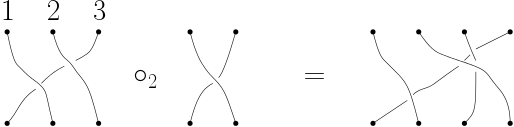
\includegraphics[scale=0.7]{Imagenes/insercion.png}
\caption{Insertion of the right braid into the second strand of the left braid.}
\end{figure}

\subsection{Operad of classifying spaces}

We have the functor of taking the nerve $N:\Cat\to\SSet$ and the functor of topological realization $|\ |:\SSet\to \CW$. One can easily check that the nerve functor behaves well with respect to the symmetric monoidal structure. Since the nerve $PaB_n$ is countable, the realization also behaves well with its symmetric monoidal structure by \ref{countable}. Let us check that the collection of cellular complexes $X_n=|N(PaB_n)|$ forms a cellular operad. Let $PaB_n'$ be the category whose objects are pairs $(x,y)$, where $x$ belongs to the braid group $B_n$ and $y$ is a parenthesizing of the non-associative product of $n$ elements, and there is a unique morphism between any two objects. We have a free left action of $B_n$ on $PaB_n':(x,y)\to (gx,y)$ and a braided operad structre on $PaB_*'$ (the structre maps are defined similarly to $PaB_n$). We have to show that the corresponding operad of classifying spaces is a topological $B_\infty$-operad and that the corresponding little disks operad is isomorphic to $X_*$ HACERLO.

Consider the corresponding chain operad. Let $C_*(PaB_n)$ be the chain complex over $\Q$ of $NPaB_n$ as a simplicial set. The collection $C_*(NPaB_n)$ forms a dg-operad (via the Eilenberg-Zilber map). We have a canonical quasi-isomorphism of operads $C_*(PaB_*)\to C_*^{sing}(|NPaB_*|)$ (just like the quasi-isomorphism between simplicial homology and singular homology). Therefore is suffices to construct a quasi-isomorphism of $C_*(PaB_*)$ and $e_2$ CAMBIAR NOTACIÓN.

\section{Operad $O_A(*)$ and construction of a quasi-isomorphism}

Let $A_n$ be the algebra over $\Q$ of power series in the noncommutative variables $t_{ij}$, where $i\geq 1$, $j\leq n$, $i\neq j$ and $t_{ij}=t_{ji}$, with relations $[t_{ij}+t_{ik},t_{kj}]=0$. Let $I_n$ be the two-sided ideal generated by all $t_{ij}$. We have a canonical projection 
\begin{equation}\label{canonical}
\pi:A_n\to A_n/I_n\cong\Q.
\end{equation}
The symmetric group $S_n$ acts naturally on $A_n$ via $\sigma\cdot t_{ij}=t_{\sigma(i)\sigma(j)}$ for $\sigma\in S_n$. The collection $\{A_n\}_{n\geq 0}$ (being $A_0$ trivial) forms an operad of algebras as we shall see. The map of the insertion into the $i$-th position $\circ_i: A_n\otimes A_m\to A_{n+m-1}$ looks as follows. Define
\[
\phi(k)=\begin{cases}
k, & k\leq i;\\
k+m-1, & k>i.
\end{cases}
\]
Then, the insertion into the $i$-th position is the linear extension of
\begin{align*}
&o_i(t_{pq}\otimes 1)=\begin{cases}
t_{\phi(p)\phi(q)}, &p,q\neq i;\\
\sum_{r=i}^{i+m-1}t_{r\phi(q)}, & p=i.
\end{cases} \\
& o_i(1\otimes t_{pq})=t_{i+p-1,i+q-1}
\end{align*}
One can verify that this map satisfies the expected propertis of the operadic composition. DEBERÍA 

Any algebra with unit over $\Q$, say $A$, gives rise to a $\Q$-additive category $C_A$ with one object. Denote by $\Q\Cat$ the category of all small $\Q$-additive categories, and by $\Q\Cat'=\Q\Cat/C_\Q$ the slice category of $\Q\Cat$ over $\C_\Q$. The objects of $\Q\Cat'$ are the elements of $\Hom(x, C_\Q)$ for each $x\in \Q\Cat'$. A morphism between $\varphi:x\to C_\Q$ and $\psi:y\to C_\Q$ is a morphism $\eta: x\to y$ in $\Q\Cat$ such that $\eta\psi=\varphi$.  This category has a clear symmetric monoidal structure obtained by the usual one on $\Cat$. We have the functor of nerve
$N^{\Q}: \Q\Cat'\to \SVect$, which is the straight analogue of the nerve of an arbitrary
category, and the functor $C_*: \SVect \to\Ch$. Both of these functors are lax monoidal (on the latter functor it is defined via the Eilenberg–Zilber map),
therefore we have a functor $\Q\Cat'\to\Ch$ and the induced functor $C_*^{\Q}:\Q\Cat'$-Operads $\to$ dg-Operads.

The map \ref{canonical} produces a morphism $\pi_*: C_{A_n}\to C_\Q$ and defines an object
$O_A(n)\in \Q\Cat'$. The operad structure on $A_n$ defines an operad structure on the
collection $\{O_A(n)\}$ TENGO QUE PENSAR ESTO. The complex $C_*^{\Q}(O_A(n))$ looks as follows. NO ME PARECE NADA EVIDENTE QUE SALGA LO QUE PONE A CONTINUACIÓN A PARTIR DE LA CONSTRUCCIÓN DEL ANTERIOR PÁRRAFO The degree $k$ component $C_k^{\Q}(O_A(n))$ is $A_n^{\otimes k}$ and the boundary map is given by
\[
d(a_1\otimes\cdots\otimes a_n)=\pi(a_1)a_2\otimes\cdots\otimes a_n-a_1a_2\otimes \cdots\otimes a_n+\cdots+(-1)^{n-1}a_1\otimes a_{n-1}\pi(a_n)
\]
COMPROBAR QUE SIN METERLE EL PI EN MEDIO VALE, PERO DE TODAS FORMAS CONSULTAR

Let $e_2$ be the operad of graded vector spaces governing the Gerstenhaber algebras NO HE VISTO QUE TAMBIÉN HAYA OPERADS EN OTRAS CATEGORÍAS QUE TAMBIÉN GENEREN LA ESTRUCTURA DE GERSTERNHABER (NO SOLO EL LITTLE DISKS).
It is generated by two binary operations: the commutative associative multiplication
of degree zero, which is denoted by $\cdot$, and the commutative bracket of degree 1
denoted by $[,]$. SUPONGO QUE ESTAS GENERARÁN IGUAL QUE LO HACEN EN EL LITTLE DISKS

These operations satisfy the Leibniz identity
\[
[ab, c]= a[b, c]+(-1)^{|b|(|c|+1)}[a,c]b
\]
and the Jacoby identity
\[
(-1)^{|a|}[a,[b,c]]+(-1)^{|a|(|b|+1)}[b,[a,c]]+(-1)^{|a||c|+|b||c|+|c|}[c,[a,b]]=0.
\]
We have a morphism of operads
\[
k:e_2\to C_*^{\Q}(O_A)
\]
which is defined on $e_2(2)$ as follows:
\[
k(\cdot)=1\in C_0^\Q(O_A),\ k([,])=t_{12}\in C_1^\Q(O_A).
\]
CREO QUE $t_{12}$ ES EL PRODUCTO POR ESTE ELEMENTO, YA QUE YENDO ATRÁS SE ESTÁ VIENDO EL ÁLGEBRA COMO UNA CATEGORÍA, PERO EN ESE CASO DEBERÍA ESPECIFICAR SI ES A IZQUIERDA O A DERECHA (QUIZÁ SOLO UNA CUMPLA LAS CONDICIONES, ASÍ QUE INTENTAR COMPROBARLO), AUN ASÍ ESTÁ MANDANDO OPERACIONES BINARIAS A OPERACIONES UNARIAS, NO LE VEO SENTIDO. Direct check shows that this map respects the relations in $e_2$ COMPROBAR.


\begin{prop}
The map $k$ is a quasi-isomorphism of operads. 
\end{prop}


DEBERÍA ESCRIBIR EN ALGÚN LADO LOS ESQUEMAS DE LAS DEMOSTRACIONES, LA GRANDE, LA DE LA FORMALDIAD, Y SI HAGO LA DE $G_\infty\to G$ TAMBIÉN
\end{document}
